

\setbeamercolor{alerted text}{fg=gray}



\tikzstyle{every picture}+=[remember picture]

\global\long\def\SO#1{\mathrm{SO}\left(#1\right)}
\global\long\def\S#1{\mathbb{S}^{#1}}
\global\long\def\sc#1{#1_{0}}
\global\long\def\vc#1{\boldsymbol{#1}}
\global\long\def\adj#1{\bar{#1}}
\global\long\def\Cn#1{\mathcal{C}_{#1}}
\global\long\def\Cd#1{\mathcal{\tilde{C}}_{#1}}
\global\long\def\Dn#1{\mathcal{D}_{#1}}
\global\long\def\Dd#1{\mathcal{\tilde{D}}_{#1}}
\global\long\def\Tn#1{\mathcal{T}_{#1}}
\global\long\def\Td{\mathcal{\tilde{T}}}
\global\long\def\On#1{\mathcal{O}_{#1}}
\global\long\def\Od{\mathcal{\tilde{O}}}


\global\long\def\Spoint{\mathcal{S}}


\global\long\def\Spointa{\tilde{\mathcal{S}}}


\global\long\def\Glaue{\mathcal{G}_{\textrm{Laue}}^{\Spoint}}


\global\long\def\Glauea{\tilde{\mathcal{G}}_{\textrm{Laue}}^{\Spoint}}


\global\long\def\I{\vc I}


\global\long\def\A{\vc A}


\global\long\def\D{\vc D}


\global\long\def\W{\vc W}
\global\long\def\V{\vc V}


\global\long\def\Id{\vc E}


\global\long\def\li{\ell}
\global\long\def\lj{\ell^{\prime}}


%\selectlanguage{english}%
\global\long\def\h#1{\hkl(#1)}
\global\long\def\u#1{\hkl[#1]}
\global\long\def\hs#1{\hkl{#1}}
\global\long\def\us#1{\hkl<#1>}



\section{grain modeling}

\subsection*{Modeling grains}

\begin{frame}[fragile]
  \frametitle{Modeling grains}

\textbf{Input:}
Spatially indexed individual orientations
given as list of tuples $\left(\vc x_{\li},p_{\li},q_{\li}\right),\li=1,\dots,n$
with
\begin{itemize}
\item locations $\vc x_{\li}\in\mathfrak{D}$ bounded to some area $\mathfrak{D}\subset\mathbb{R}^{d}$,
\item phase information $p_{\li}\in\mathbb{N}^{+}$ (includes crystal symmetry),
\item orientations $q_{\li}\in\SO 3$.
\end{itemize}

\textbf{Output:}
A graph based data model representing grains and grain boundaries.

\end{frame}


\begin{frame}[fragile]
  \frametitle{Modeling grains}

\begin{overprint}

\onslide<1>
\begin{center}
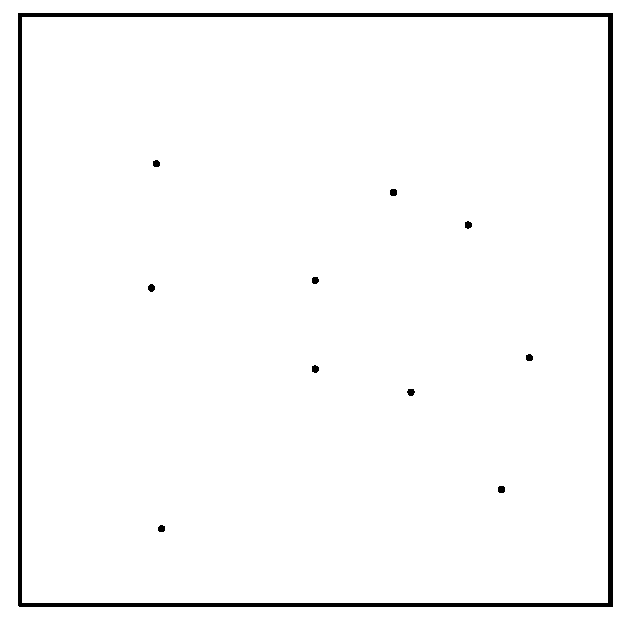
\includegraphics[height=0.9\textheight]{fig/voronoi-x}
\par\end{center}

\onslide<2>
\begin{center}
\includegraphics[height=0.9\textheight]{fig/voronoi-b1}
\par\end{center}

\onslide<3>
\begin{center}
\includegraphics[height=0.9\textheight]{fig/voronoi-b1}
\par\end{center}


\onslide<4>
\begin{center}
\includegraphics[height=0.9\textheight]{fig/voronoi-b2}
\par\end{center}

\onslide<5>
\begin{center}
\includegraphics[height=0.9\textheight]{fig/voronoi-b3}
\par\end{center}


\onslide<6>
\begin{center}
\includegraphics[height=0.9\textheight]{fig/voronoi-b4}
\par\end{center}

\onslide<7>
\begin{center}
\includegraphics[height=0.9\textheight]{fig/voronoi-b5}
\par\end{center}

\onslide<8>
\begin{center}
\includegraphics[height=0.9\textheight]{fig/voronoi-b6}
\par\end{center}



\onslide<9>
\begin{center}
\includegraphics[height=0.9\textheight]{fig/voronoi-v1}
\par\end{center}


\onslide<10>
\begin{center}
\includegraphics[height=0.9\textheight]{fig/voronoi-v2}
\par\end{center}




\onslide<11>
\begin{center}
\includegraphics[height=0.9\textheight]{fig/voronoi-v2}
\par\end{center}


\onslide<12>
\begin{center}
\includegraphics[height=0.9\textheight]{fig/voronoi-iom-ad}
\par\end{center}


\onslide<13>
\begin{center}
\includegraphics[height=0.9\textheight]{fig/voronoi-iom-adpm}
\par\end{center}


\onslide<14>
\begin{center}
\includegraphics[height=0.9\textheight]{fig/voronoi-iom-adpmg}
\par\end{center}


\onslide<15>
\begin{center}
\includegraphics[height=0.9\textheight]{fig/voronoi-iom-adpmgs}
\par\end{center}


\onslide<16>
\begin{center}
\includegraphics[height=0.9\textheight]{fig/voronoi-iom-adpmgsb}
\par\end{center}


\onslide<17>
\begin{center}
\includegraphics[height=0.9\textheight]{fig/voronoi-iom-f}
\par\end{center}

\end{overprint}

\end{frame}


\begin{frame}[fragile]
  \frametitle{Modeling grains: algorithm}


% \tikzstyle{na} = [baseline=-.5ex]
\tikzset{Ive/.style ={anchor=base,fill=none},%
         Ied/.style ={anchor=base,fill=none},%
         Idg/.style ={anchor=base,fill=none},%
         Ag/.style ={anchor=base,fill=none},%
         Ad/.style = {anchor=base,fill=none},%
         Ams/.style ={anchor=base,fill=none},%
         Aps/.style ={anchor=base,fill=none},%
         Apg/.style ={anchor=base,fill=none},%
         Apgs/.style ={anchor=base,fill=none}}
\only<2>{\tikzset{Ive/.style ={anchor=base,fill=yellow}}}
\only<3>{\tikzset{Ied/.style ={anchor=base,fill=yellow}}}
\only<9>{\tikzset{Idg/.style ={anchor=base,fill=yellow}}}
\only<11>{\tikzset{Ag/.style ={anchor=base,fill=yellow}}}
\only<4>{\tikzset{Ad/.style ={anchor=base,fill=yellow}}}
\only<6>{\tikzset{Ams/.style ={anchor=base,fill=red!30}}}
\only<7>{\tikzset{Aps/.style ={anchor=base,fill=green!30}}}
\only<14>{\tikzset{Apgs/.style ={anchor=base,fill=blue!30}}}
\only<15>{\tikzset{Apg/.style ={anchor=base,fill=green!30}}}
\begin{overlayarea}{\textwidth}{\textheight}
\begin{enumerate}
\item <1-|alert@5->Voronoi-decomposition resulting in incidence matrix
$\tikz[baseline]{\node[Ive](ive){\ensuremath{\I_{VE}}};},
\tikz[baseline]{\node[Ied](ied){\ensuremath{\I_{ED}}};}$
and adjacency matrix
 $\tikz[baseline]{\node[Ad](aa){\ensuremath{\A_{D}}};}$.\only<2>{ {\footnotesize
\[
\left[\tikz[baseline]{\node[Ive](ve){\ensuremath{\I_{VE}}};}\right]^{i,j}=\begin{cases}
1, & \mbox{if vertex }v _{i}\mbox{ incident to edge }e_{j},\\
0, & \mbox{otherwise}.
\end{cases}
\]
}}\only<3>{ {\footnotesize
\[
\left[\tikz[baseline]{\node[Ied](ed){\ensuremath{\I_{ED}}};}\right]^{j,\li}=\begin{cases}
1, & \mbox{if edge }e _{j}\mbox{ incident to Voronoi-cell }D(\vc{x}_{\li}),\\
0, & \mbox{otherwise}.
\end{cases}
\]
}}\only<4>{ {\footnotesize
\[
\left[\tikz[baseline]{\node[Ad](ad){\ensuremath{\A_{D}}};}\right]^{\li,\lj}=\begin{cases}
1, & \mbox{if Voronoi-cell }D(\vc{x}_{\li})\mbox{ adjacent to Voronoi-cell }D(\vc{x}_{\lj}),\\
0, & \mbox{otherwise}.
\end{cases}
\]
}}
\item <5-|alert@8->Decompose adjacencies $\A_{D}=\tikz[baseline]{\node[Ams](Am){\ensuremath{\A_{D}^{\circ}}};}+\tikz[baseline]{\node[Aps](Ap){\ensuremath{\A_{D}^{\partial}}};}$\only<2>{.}\only<6>{,{\footnotesize
\[
\left[\tikz[baseline]{\node[Ams](am){\ensuremath{\A_{D}^{\circ}}};}\right]^{\li,\lj}=\begin{cases}
1, & \mbox{if }D\left(\vc x_{\li}\right)\mbox{ and }D\left(\vc x_{\lj}\right)\mbox{ adjacent and {\color{red}no\,\ grain boundary}},\\
0, & \mbox{otherwise}.
\end{cases}
\]
}}\only<7>{,{\footnotesize
\[
\left[\tikz[baseline]{\node[Aps](ap){\ensuremath{\A_{D}^{\partial}}};}\right]^{\li,\lj}=\begin{cases}
1, & \mbox{if }D\left(\vc x_{\li}\right)\mbox{ and }D\left(\vc x_{\lj}\right)\mbox{ adjacent and {\color{green}grain boundary}},\\
0, & \mbox{otherwise}.
\end{cases}
\]
}}\only<9->{.}
\item <8-|alert@11->Search components of $\A_{D}^{\circ}$
via depth-first search and determine incidence matrix $\tikz[baseline]{\node[Idg](idg){\ensuremath{\I_{DG}}};}
\subseteq D\times G$\only<9>{,{\footnotesize
\[
\left[\tikz[baseline]{\node[Idg](dg){\ensuremath{\I_{DG}}};}\right]^{\li,m}=\begin{cases}
1, & \mbox{if }D\left(\vc x_{\li}\right)\mbox{ is part of grain }g_{m},\\
0, & \mbox{otherwise}.
\end{cases}
\]
}}\only<10->{.}
\item <10-|alert@13->Represent adjacencies of grains in a matrix $\tikz[baseline]{\node[Ag](aga){\ensuremath{\A_{G}}};}\subseteq G\times G$\only<11>{, {\footnotesize
\[
\left[\tikz[baseline]{\node[Ag](ag){\ensuremath{\A_{G}}};}\right]^{m,m^{\prime}}=\begin{cases}
1, & \mbox{if grain }g_{m}\mbox{ and }g_{m^{\prime}}\mbox{ have a common grain boundary},\\
0, & \mbox{otherwise}.
\end{cases}
\]
}}\only<12>{,{\footnotesize
\[
\left[\A_{G}\right]^{m,m^{\prime}}=\begin{cases}
1, & \mbox{if }\left[\I_{DG}^{\top}\A_{D}^{\partial}\I_{DG}\right]^{m,m^{\prime}}>0,\\
0, & \mbox{otherwise}.
\end{cases}
\]
}}\only<13->{.}
\item <13-|alert@16->Decompose adjacencies $\A_{D}^{\partial}=\tikz[baseline]{\node[Apgs](Apgs){\ensuremath{\A_{D}^{\partial_{\mathrm{sub}}}}};}+\tikz[baseline]{\node[Apg](Apg){\ensuremath{\A_{D}^{\partial_{\mathrm{ext}}}}};}$\only<14>{.}\only<14>{,{\footnotesize
\[
\left[\tikz[baseline]{\node[Apgs](apgs){\ensuremath{\A_{D}^{\partial_{\mathrm{sub}}}}};}\right]^{\li,\lj}=\begin{cases}
1, & \mbox{if }D\left(\vc x_{\li}\right)\mbox{ and }D\left(\vc x_{\lj}\right)\mbox{ adjacent and {\color{blue}sub grain boundary}},\\
0, & \mbox{otherwise}.
\end{cases}
\]
}}\only<15>{,{\footnotesize
\[
\left[\tikz[baseline]{\node[Apg](apg){\ensuremath{\A_{D}^{\partial_{\mathrm{ext}}}}};}\right]^{\li,\lj}=\begin{cases}
1, & \mbox{if }D\left(\vc x_{\li}\right)\mbox{ and }D\left(\vc x_{\lj}\right)\mbox{ adjacent and {\color{green}grain boundary}},\\
0, & \mbox{otherwise}.
\end{cases}
\]
}}\only<16>{.}
\item <16-|alert@17->Compute incidence matrix $\I_{EG}=\I_{ED}\I_{DG}$ and  decompose
$\I_{EG}=\I_{EG}^{\circ}+\I_{EG}^{\partial}$, with $\I_{EG}^{\partial}=\I_{EG}^{\partial_{\mathrm{sub}}}+\I_{EG}^{\partial_{\mathrm{ext}}}$.
\end{enumerate}
\only<17->{\textbf{Output}:\\
$\A_{D}^{\circ},\,\A_{D}^{\partial_{\mathrm{sub}}},\,\A_{D}^{\partial_{\mathrm{ext}}},\A_{G},$\\
$\I_{DG},\,\I_{ED}^{\partial_{\mathrm{sub}}},\,\I_{ED}^{\partial_{\mathrm{ext}}},$\\}
\end{overlayarea}
% have to apply the 'overlay' style.
\begin{tikzpicture}[overlay]
   \path[->]<2> (ve) edge [out=60, in=-150,yellow,line width=2pt] (ive);
   \path[->]<3> (ed) edge [out=60, in=-150,yellow,line width=2pt] (ied);
   \path[->]<4> (ad) edge [out=60, in=-150,yellow,line width=2pt] (aa);
   \path[->]<6> (am) edge [out=60, in=-150,red!30,line width=2pt] (Am);
   \path[->]<7> (ap) edge [out=45, in=-150,green!30,line width=2pt] (Ap);
   \path[->]<9> (dg) edge [out=90, in=-120,yellow,line width=2pt] (idg);
   \path[->]<11> (ag) edge [out=45, in=-150,yellow,line width=2pt] (aga);
   \path[->]<14> (apgs) edge [out=45, in=-150,blue!30,line width=2pt] (Apgs);
   \path[->]<15> (apg) edge [out=45, in=-150,green!30,line width=2pt] (Apg);
\end{tikzpicture}

\end{frame}


\begin{frame}[fragile]
  \frametitle{Modeling grains: algorithm}


\textbf{Benefits ... }
\begin{itemize}
\item Works in 2d and 3d
\item Voronoi-decomposition flexible against not indexed data
\item No interpolation of orientation
\item Explicit data model ensures fast access to adjacencies and incidences.
\item Almost every spatial relationship of EBSD data and its grains can be represented.
\end{itemize}


\textbf{... Disadvantages}
\begin{itemize}
\item Voronoi-decomposition is expensive.
\item Large memory costs to store all adjacencies and incidences.
\end{itemize}

\end{frame}



\subsection*{Modeling grains}

\begin{frame}[fragile]
  \frametitle{Modeling grains}


\begin{overprint}

\onslide<1>

\begin{lstlisting}
mtexdata mylonite
plot(ebsd,'property','phase');
\end{lstlisting}

\begin{center}
\includegraphics[width=\linewidth]{fig/twinsa}
\par\end{center}


\onslide<2>
\begin{lstlisting}
grains = calcGrains(ebsd,'angle',5*degree);
hold on, plotBoundary(grains);
\end{lstlisting}

\begin{center}
\includegraphics[width=\linewidth]{fig/twinsb}
\par\end{center}



\onslide<3>
\begin{lstlisting}
plot(grains,'property','phase')
\end{lstlisting}

\begin{center}
\includegraphics[width=\linewidth]{fig/twinsd}
\par\end{center}


\onslide<4>
\begin{lstlisting}
hold on, plotBoundary(grains,'property',...
   orientation(...));
\end{lstlisting}


\begin{center}
\includegraphics[width=\linewidth]{fig/twinsc}
\par\end{center}

\end{overprint}

\end{frame}



\subsection{Properies of grains}
\begin{frame}[fragile]
  \frametitle{Properties of grains}

\textbf{Incidencies and Adjacencies}
\begin{lstlisting}
get(grains,'I_VF')
get(grains,'I_DG')
get(grains,'I_FG')
get(grains,'I_FDext')
get(grains,'I_FDint')
get(grains,'A_D')
get(grains,'A_G')
\end{lstlisting}

\textbf{Properties}
\begin{lstlisting}
get(grains,'EBSD')
get(grains,'orientation')
get(grains,'orientations')
get(grains,'...')
\end{lstlisting}

\end{frame}




\subsection{Properies of grains}
\begin{frame}[fragile]
  \frametitle{Properties of grains}

\textbf{Geometric properties of grains}
\begin{lstlisting}
area(grains)
perimeter(grains)
diameter(grains)
centroid(grains)
shapefactor(grains)
aspectratio(grains)
equivalentradius(grains)
equivalentperimeter(grains)
principalcomponents(grains)
...
\end{lstlisting}

\textbf{Other properties}
\begin{lstlisting}
grainSize(grains)
hasHole(grains)
isNotIndexed(grains)
\end{lstlisting}

\end{frame}


\subsection{Accessing grains}
\begin{frame}[fragile]
  \frametitle{Acessing grains}

\textbf{Accessing by phase}
\begin{lstlisting}
grains('mineral name')
grains({'fe','mg'})
\end{lstlisting}

\textbf{Accessing grains by indexing or logical expression}
\begin{lstlisting}
grains(1)
grains(1:10)
grains( area(grains) > 100 )
grains(diameter(grains)>10 | perimeter(grains)>10)
grains(diameter(grains)>10 & grains('fe'))
grains(grainSize(grains)>1 & ~grains('notindexed'))
\end{lstlisting}

\textbf{Concatenation of grain}
\begin{lstlisting}
[grains('fe') grains('mg')]
\end{lstlisting}
\end{frame}


\subsection{Correcting EBSD and grains}
\begin{frame}[fragile]
  \frametitle{Correcting EBSD and grains}

\begin{overlayarea}{\linewidth}{8cm}
\only<1-2>{
\begin{center}
\only<1>{\includegraphics[width=\linewidth]{fig/ebsd_correction_1a}}
\only<2>{\includegraphics[width=\linewidth]{fig/ebsd_correction_1b}}
\par\end{center}
\begin{enumerate}
\item <1->Import EBSD.
\item <2-> Reconstruct grains.
\end{enumerate}
% \vspace*{\fill}
}

\only<3-5>{
\begin{center}
\only<3>{\includegraphics[width=\linewidth]{fig/ebsd_correction_1a}}
\only<4>{\includegraphics[width=\linewidth]{fig/ebsd_correction_2b}}
\only<5>{\includegraphics[width=\linewidth]{fig/ebsd_correction_2c}}
\par\end{center}
\begin{enumerate}
\item <3->Import EBSD.
\item <4->Remove badly indexed data and remove non-plausible grains, e.g. '1-pixel' grains.
\item <5->Reconstruct grains.
\end{enumerate}
% \vspace*{\fill}
}

\only<6-9>{
\begin{center}
\only<6>{\includegraphics[width=\linewidth]{fig/ebsd_correction_1a}}
\only<7>{\includegraphics[width=\linewidth]{fig/ebsd_correction_3b}}
\only<8>{\includegraphics[width=\linewidth]{fig/ebsd_correction_3c}}
\only<9>{\includegraphics[width=\linewidth]{fig/ebsd_correction_3d}}
\par\end{center}
\begin{enumerate}
\item <6->Import EBSD.
\item <7->Reconstruct grains.
\item <8->Remove non-plausible data but keep some dummy data.
\item <9->Reconstruct grains again.
\end{enumerate}
% \vspace*{\fill}
}



% Data correction is important!\\
% \textbf{Your first exercise when analysing ebsd: correct it.}}
\end{overlayarea}
\end{frame}



\subsection{Grain boundaries and misorienation}
\begin{frame}[fragile]
  \frametitle{Grain boundaries and misorienation}



\begin{overprint}
\onslide<1>
\textbf{via boundary misorientation angular distribution} %\vspace*{-.45cm}
\begin{lstlisting}
plotAngleDistribution(grains)
plotAngleDistribution(grains('fe'),63)
plotAngleDistribution(grains('fe'),grains('mg'),63)
\end{lstlisting}
\begin{center}
\includegraphics[width=7cm]{fig/grains_angledistribution}
\par\end{center}


\onslide<2>
\textbf{via boundary misorientation axis distribution} %\vspace*{-.45cm}
\begin{lstlisting}
plotAxisDistribution(grains('fe'))
plotAxisDistribution(grains('mg'),...
                         'smooth','antipodal')
plotAxisDistribution(grains('mg'),grains('fe'))
\end{lstlisting}
\begin{center}
\includegraphics[width=.3\linewidth]{fig/grains_axisdistribution_fe}
\includegraphics[width=.3\linewidth]{fig/grains_axisdistribution_mg}
\includegraphics[width=.3\linewidth]{fig/grains_axisdistribution_mg_fe}
\par\end{center}


\onslide<3->
\textbf{via spatial plots}%\vspace*{-.45cm}
\begin{lstlisting}
plotBoundary(grains,'property','angle')
plotBoundary(grains,'property','misorientation')
plotBoundary(grains,'property',...
   orientation(...),'delta',2*degree)
plotBoundary(grains,'property',[2 10]*degree)

\end{lstlisting}
\begin{center}
\only<3>{\includegraphics[width=\linewidth]{fig/grains_boundary_angle}}%
\only<4>{\includegraphics[width=\linewidth]{fig/grains_boundary_misorientation}}%
\only<5>{\includegraphics[width=\linewidth]{fig/grains_boundary_special}}%
\only<6>{\includegraphics[width=\linewidth]{fig/ebsd_boundary_1a}}%
\par\end{center}
\end{overprint}

\end{frame}


\subsection{Grains and interal misorienation}
\begin{frame}[fragile]
  \frametitle{Grains and internal misorienation}



\begin{overprint}
\onslide<1-2>
\textbf{Observe misorientation within a grain} %\vspace*{-.45cm}
\begin{lstlisting}
plot(grains,'property','mis2mean')
plot(grains,'property','mis2mean',...
                    'colorcoding','angle')
\end{lstlisting}
\begin{center}
\only<1>{\includegraphics[width=\linewidth]{fig/grains_mis2mean}}%
\only<2>{\includegraphics[width=\linewidth]{fig/grains_mis2mean_angle}}
\par\end{center}


\onslide<3-5>
\begin{overlayarea}{\linewidth}{10cm}
\textbf{Observe misorientation of grains individually} %\vspace*{-.45cm}

\begin{lstlisting}
singlegrain = findByLocation(grains,[x y])
plotKAM(singlegrain)
spatialProfile(singlegrain,[x1 y1; x2 y2])
\end{lstlisting}
\begin{center}
\vspace*{-.5cm}
\only<3>{\includegraphics[width=\linewidth]{fig/grains_misorientation_1a}}%
\only<4->{\includegraphics[width=\linewidth]{fig/grains_misorientation_1b}}%
\vspace*{-.8cm}
\hspace*{1.4cm}\only<5>{
\includegraphics[width=.7\linewidth]{fig/grains_misorientation_1c}}%
\par\end{center}
\end{overlayarea}
\end{overprint}

\end{frame}




\subsection{Grains and misorienation}
\begin{frame}[fragile]
  \frametitle{Grains and misorienation}

\begin{overprint}
\onslide<1>
\textbf{via boundary misorientation angular distribution} %\vspace*{-.45cm}
\begin{lstlisting}
plotAngleDistribution(grains)
plotAngleDistribution(grains('fe'),63)
plotAngleDistribution(grains('fe'),grains('mg'),63)
\end{lstlisting}
\begin{center}
\includegraphics[width=7cm]{fig/grains_angledistribution}
\par\end{center}

\end{overprint}
\end{frame}

\only<3>{
\begin{lstlisting}
plotBoundary(grains,'property','angle')
plotBoundary(grains,'property','misorientation')
plotBoundary(grains,'property',...
   orientation(...),'delta',2*degree)
\end{lstlisting}
}

% \only<4>{
% \textbf{Analyze via misorientations}
% \begin{lstlisting}
% m = calcMisorientation(grains('fe'),grains('mg'))
% axis(m);
% angle(m)/degree;
% \end{lstlisting}

% \textbf{Your exercise}: \texttt{mtexdata mylonite}
% Classify and plot special boundaries
% }

% \end{overprint}
% \end{frame}



\subsection{Organizing grains hierarchically}
\begin{frame}[fragile]
  \frametitle{Organizing grains hierarchically}


\begin{overprint}
\onslide<1>
\textbf{merging grains with certain misorientation angle}
\begin{lstlisting}
[grains5  I_5]  = merge(grains,5*degree);
[grains10 I_10] = merge(grains5,10*degree);

sum(I_5,2); sum(I_10,2);
sum(I_10*I_5,2);
\end{lstlisting}

\onslide<2->
\textbf{merging grains with special boundary}
\begin{lstlisting}
[grains_csl I_csl] = merge(grains,CSL(3));
[grains_o   I_o  ] = merge(grains,...
             orientation(...),'delta',2*degree);
\end{lstlisting}


\begin{center}
\vspace*{-.5cm}
\only<2>{\includegraphics[width=\linewidth]{fig/grains_merge_1a}}%
\only<3>{\includegraphics[width=\linewidth]{fig/grains_merge_1b}}%
\only<4>{\includegraphics[width=\linewidth]{fig/grains_merge_1c}}%
\only<5>{\includegraphics[width=\linewidth]{fig/grains_merge_1d}}%
\par\end{center}

\end{overprint}
\end{frame}


% \section{Grains}


% \subsection{reconstruction of grains}
% \begin{frame}
%   \frametitle{Reconstruction of grains}

% \end{frame}


% \begin{frame}
%   \frametitle{Accessing grains}




% \end{frame}

% \subsection{grain boundary analysis}

% \subsection{Plotting grain boundaries}
% \begin{frame}
%   \frametitle{Plotting grain boundaries}


% \end{frame}


% \begin{frame}
%   \frametitle{misorientation at grain boundaries}




% \end{frame}



% \subsection{Merging grains}
% \begin{frame}
%   \frametitle{Organizing grains}

% merge


% \end{frame}




\subsection{Exercises}
\begin{frame}
  \frametitle{Exercises}

 Examine the EBSD data \textcolor{blue}{\texttt{mtexdata aachen}}:
  \begin{itemize}
  \item Correct the EBSD data / grains.
  \item How does the correction influence the data analysis?
  \end{itemize}

 Examine the EBSD data \textcolor{blue}{\texttt{mtexdata mylonite}}:

  \begin{itemize}
  \item Characterize special grain boundaries for all phases.
  \item Visualize your results.
  \end{itemize}

  Examine the EBSD data \textcolor{blue}{\texttt{ebsd\_mergeCSL3.txt}}:

  \begin{itemize}
  \item Which texture is present?
  \item Characterize special grain boundaries.
  \item Merge grains and investigate merged regions.
  \item What is wrong with the data?
  \end{itemize}


\end{frame}


% \begin{frame}

% \begin{center}
% \includemovie[poster,toolbar,label=grains_vox,text=(5 largest grains),3Dviews2=pic/views.txt,3Djscript=pic/grains_explode.js]{11cm}{8cm}{pic/grains_vox.u3d}
% \end{center}

% \end{frame}



%  \begin{frame}

% \begin{center}
% \includemovie[poster,toolbar,label=grains_smooth,text=(5 largest grains),3Dviews2=pic/views.txt,3Djscript=pic/grains_explode.js]{11cm}
% {8cm}{pic/grains_smooth.u3d}
% \end{center}

%  \end{frame}


% \begin{frame}

% \begin{center}
% \includemovie[poster,toolbar,label=grains_smooth2,text=(5 largest grains),3Dviews2=pic/views.txt,3Djscript=pic/grains_explode.js]{11cm}{8cm}{pic/grains_smooth2.u3d}
% \end{center}

% \end{frame}



%%% Local Variables:
%%% mode: latex
%%% TeX-master: "main"
%%% End:
